% dtmf-en-de.tex
% This is the whole document about DTMF encoder and decoder.

\documentclass[11pt,a4paper]{article}

\usepackage{graphicx}
\usepackage{indentfirst}
\usepackage{verbatim}
%\usepackage{multirow}
%\usepackage{fancybox}
%\usepackage{endnotes}

\title{DTMF Encoder and Decoder: PWM of ATmega48}
\author{sun\_ge@yahoo.cn}

\begin{document}

\maketitle


\section{Project Origin}
I noticed that many \em{Smart Home} projects based on DTMF communication between telephone
and microcontroller. So I tried to do some experiment about DTMF.
I use ATmega48 to generate DTMF signal then decode it with LC7385 decoder, because:
\begin{enumerate}
\item ATmega48's 8-bit PWM output is suitable to generate DTMF tones.
\item It has sufficient GPIO to read a 4x4 keypad and drive a LCD.
\item ATMEL provide a application note ~\textit{AVR314: DTMF Generator}~ and
example code~\textit{DTMF.C}.
\item LC7385 can testify the DTMF tone which ATmega48 generated whether available or not.
\end{enumerate}

\section{DTMF Encoder(Generator)}
\begin{center}
You can enlarge the picture.\\
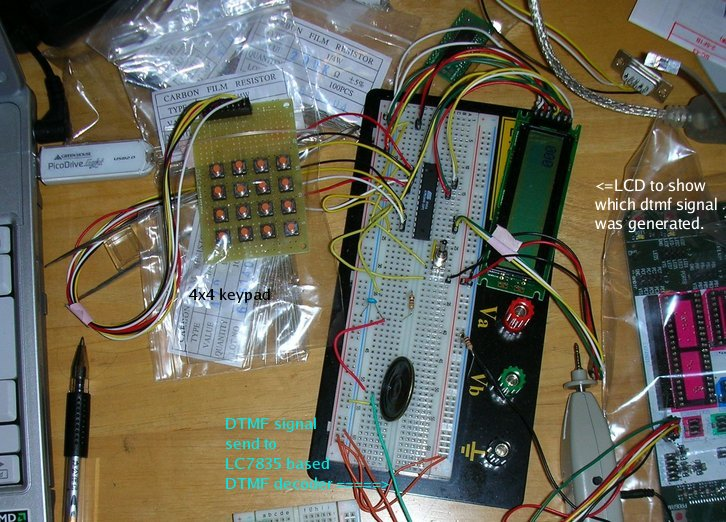
\includegraphics[scale=0.8]{dtmf-en.jpg}
\end{center}

\subsection{Hardware}
The following is the connection of hardware:
\verbatiminput{connect.txt}

Instead of schematics, source code also contains hardware informations
and technical notes, please read it for details.\\


\subsection{Source Code}
Source contains: lcd.h, lcd.c, KPDScan.h, KPDScan.c, dtmf.c and Makefile.\\
It can be compiled and installed by AVR GNU Tools Chain.

\subsubsection{LCD Library Header: lcd.h}
\verbatiminput{lcd.h}

\subsubsection{LCD Library: lcd.c}
\verbatiminput{lcd.c}

\subsubsection{Keypad Library Header: KPDScan.h}
\verbatiminput{KPDScan.h}

\subsubsection{Keypad Library: KPDScan.c}
\verbatiminput{KPDScan.c}

\subsubsection{Main Program: dtmf.c}
\verbatiminput{dtmf.c}

\subsubsection{Makefile}
\verbatiminput{Makefile}

\section{DTMF Decoder}
\begin{center}
You can enlarge the picture.\\
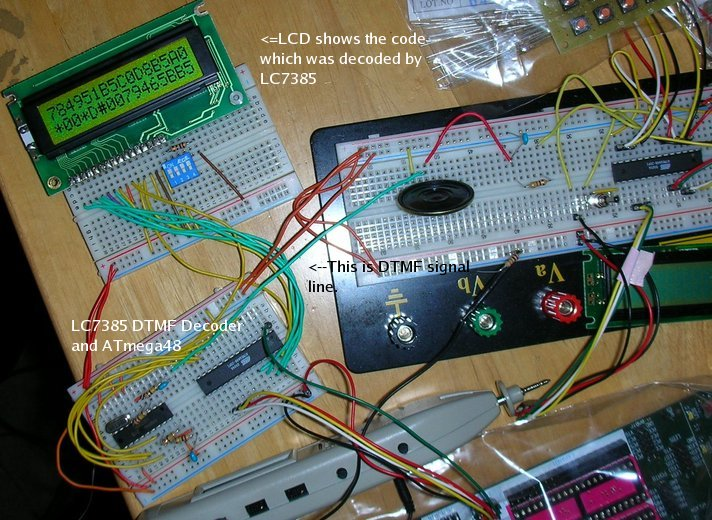
\includegraphics[scale=0.8]{../dtmf-decoder/dtmf-de.jpg}
\end{center}

\subsection{Hardware}
The following is the connection of hardware:
\verbatiminput{../dtmf-decoder/connect.txt}

\subsection{Source Code}
Source contains: lcd.h, lcd.c, dtmf2.c and Makefile.\\
\subsubsection{LCD Library Header: lcd.h}
\verbatiminput{../dtmf-decoder/lcd.h}

\subsubsection{LCD Library: lcd.c}
\verbatiminput{../dtmf-decoder/lcd.c}

\subsubsection{Main Program: dtmf2.c}
\verbatiminput{../dtmf-decoder/dtmf2.c}

\subsubsection{Makefile}
\verbatiminput{../dtmf-decoder/Makefile}

\end{document}
%%% Local Variables:
%%% coding: UTF-8
%%% mode: latex
%%% End:
